\chapter[\hspace{0pt}问题重述]{{\heiti\zihao{3}\hspace{0pt}问题重述}}\label{chapter: 问题重述}

本章内容共分为四节,\hyperref[section1: 问题一]{第一节}介绍本文的研究背景及意义;\hyperref[section1: 问题二]{第二节}总结少样本分类算法的国内外研究现状,并对其面临的挑战进行分析;\hyperref[section1: 问题三]{第三节}介绍本文的研究内容与创新点;\hyperref[section1: 本文组织结构]{第四节}对本文组织结构进行概括。

\section[\hspace{-2pt}问题一]{{\heiti\zihao{-3} \hspace{-8pt}问题一}}\label{section1: 问题一}

在当今时代,深度学习技术已在诸如图像分类、目标检测、实例分割等人工智能领域中取得显著成就\cite{krizhevsky2012imagenet, yolo, FasterRcnn, MaskRcnn, 图像分类, 陈科圻2020多尺度目标检测的深度学习研究综述, 蒋弘毅2021目标检测模型及其优化方法综述, 语义分割},在某些特定任务中的表现达到甚至超越了人类的水平。然而,这些技术的成功在很大程度上依赖于大规模标注数据集的支撑。一旦没有足够数量的标注样本,很多深度学习模型便会因为只在少量样本数据上进行训练而出现过拟合或欠拟合现象,进而导致无法达到良好的性能表现。

与深度学习模型不同,人类在成长过程中学习积累了大量知识后,面对新物体或新场景时能够总结以往的知识与经验,通过少量样本便可迅速准确地识别新类别。例如,某人已经认识了“猫”、“狗”、“马”等动物,而从未见过“水豚”这类动物,但通过观察几张甚至一张“水豚”的图片,便可对其准确识别,而深度学习模型则可能需要使用数百乃至上千张图片进行训练才能达到相同的识别效果。为了模拟人类认识新类别的过程,少样本分类(Few-Shot Classification, 简称FSC)应运而生。少样本分类致力于模拟人类的知识迁移能力,期望模型在具有大量标注数据的基类数据上训练之后,能够将所学知识迁移至新类别上,实现用少量标注样本进行有效学习。

作为目前计算机视觉领域的热门研究方向之一,无论是在学术探索还是实际应用方面,少样本分类都具有深远意义。首先,在学术探索方面,少样本分类打破了传统深度学习依赖大规模标注数据集进行训练的范式,推动了包括元学习、迁移学习、模型正则化等在内的一系列理论和方法的发展,为解决深度学习任务中的数据稀缺问题提供了新的视角和方法论。并且少样本分类强调模型的泛化能力,为提高模型在仅有少量标注数据类别上的泛化性能,多种理论和算法被提出,这同样可被其他学习任务借鉴使用。另外,在现实场景中,诸多任务无法获取大量标注数据,少样本分类为这些任务提供了理论基础和技术支持。例如,医学图像分析、疾病诊断领域,标注数据获取困难且成本高昂。少样本分类技术可以利用有限的病例进行高效学习,辅助医生进行更准确的诊断。在生态研究和动物识别等领域,很多物种稀有导致难以收集大量样本,少样本分类可以帮助识别这类物种。

少样本分类需要在大量标注数据的基类上训练之后,在仅有少量标注数据的新类上执行分类任务,因此如何迁移学习到的知识成为了关键。虽然基类与新类的样本类别不同,但其数据间却共享着一些深层次、多样化的关系,这些关系表现为样本间的相似性、差异性,以及语义空间与视觉空间的联系性等。通过在基类数据上对这些关系进行建模,可以更好地理解与挖掘数据间的内在联系,从而迁移在基类上学习到的知识,提升模型在新类数据上的表现。本文旨在研究少样本数据集中的多元关系,通过建模多粒度样本关系,提升视觉特征提取网络的特征提取能力和视觉特征的判别性;通过引入语义信息,建模语义-视觉多空间关系,使得模型可以获取标注样本的多种模态信息,提高模型的泛化能力。本文充分挖掘并利用样本数据的多元关系,为少样本分类问题提供了新的研究视角,有望为少样本分类领域的学术研究与实际应用进程起到一定程度的促进作用。


\section[\hspace{-2pt}问题二]{{\heiti\zihao{-3} \hspace{-8pt}问题二}}\label{section1: 问题二}

\subsection[\hspace{-2pt}研究现状]{{\heiti\zihao{4} \hspace{-8pt}研究现状}}\label{section1: 研究现状}

近年来,已有很多少样本分类方法被提出,按其技术方案可以大致分为五类,分别是:基于元学习的少样本算法、基于度量的少样本算法、基于数据增强的少样本算法、基于特征学习的少样本算法和基于语义的少样本算法,以下将分别对其进行介绍。

\textbf{(1)基于元学习的少样本算法}

基于元学习的少样本分类算法\cite{MAML, lee2019meta, LEO, 元学习},其核心思想是在训练阶段便模拟少样本测试任务,在从基类数据集采样的大量少样本分类任务中学习到元知识,元知识可以迁移到其他少样本任务,从而使模型在遇到新任务时能够通过极少量的样本训练便快速调整参数并达到较好的分类性能。例如,Finn等人\cite{MAML}提出了模型无关的元学习算法(Model-Agnostic Meta-Learning,简称 MAML)。MAML设计了一种优化算法,通过找到一组初始化模型参数,使用少量梯度下降便能够使其适应新的任务。Lee等人\cite{lee2019meta}则是使用支持向量机(Support Vector Machine,简称SVM)代替MAML方法中的线性分类器,并结合了一个可微分二次规划求解器使得其能够端到端学习。Rusu等人\cite{LEO}提出了一种在低维潜在空间进行模型元学习的方法LEO,其将元学习问题转化为潜在空间中的优化问题,利用潜在空间的特征嵌入捕捉少样本任务间共享的结构性知识,促进不同任务间的知识转移。基于元学习的方法虽很符合少样本分类的特点,但其通常需要先对特征提取网络进行预训练,并在元学习阶段采样大量任务来微调网络,存在训练过程较为复杂的问题。

\textbf{(2)基于度量的少样本算法}

基于度量的方法\cite{ProtoNet, vinyals2016matching, DeepEMD, 度量学习}为少样本分类问题提供了另一种解决思路,其旨在通过学习样本之间的距离或相似度度量来处理少样本问题。这类方法的核心思想是,如果能够合理地度量样本之间的距离或相似性,即便是只有少量的训练样本,也可以通过比较未知样本与已知样本之间的距离或相似度来进行有效的分类。基于度量的方法大多使用欧式距离、余弦相似度计算样本之间的距离,例如Snell等人\cite{ProtoNet}提出的原型网络(Prototypical Networks, 简称ProtoNet)。ProtoNet基于以下假设:在特征空间中,每个类别都可以由其样本特征的平均值代表的一个原型来表示。在进行分类时,其会计算查询样本与每个类别原型之间的欧式距离,并将查询样本分类到最近的原型所代表的类别。Zhang等人\cite{DeepEMD}提出的DeepEMD方法为少样本分类引入了一种新的距离度量方式:推土机距离(Earth Mover's Distance,简称EMD)。DeepEMD将一张图像分为不同的图像块,对其进行特征提取并利用推土机距离作为度量标准来比较不同图像之间的相似度。另外,Sung等人\cite{RelationNet}提出的关系网络(Relation Networks,简称RelationNet)则是通过学习一个深度度量来评估样本之间的关系得分,进而通过关系得分进行分类。与之前方法不同,此关系得分是通过网络学习到的,而不是设计的固定距离度量方式。基于度量的少样本算法简单高效,其难点主要在于如何建立一个合适的度量方式来衡量样本之间的距离或相似度。

\textbf{(3)基于数据增强的少样本算法}

增加样本数量来应对标注样本不足的问题,是少样本分类最直观的解决方案,因此,基于数据增强的少样本算法被提出\cite{IDeMe-Net, AFHN}。少样本分类中,每个类别样本数目极少,模型很容易产生过拟合问题,该类算法通过增加训练样本的数量和多样性来帮助模型学习到更加鲁棒的特征表示,从而减少过拟合的风险。例如,Chen等人\cite{IDeMe-Net}提出了一种名为图像变形元网络(Image Deformation Meta-Networks,简称IDeMe-Net)的新颖框架。IDeMe-Net训练一个网络,该网络能够通过线性地融合一组图像生成变形图像,从而产生额外的标注样本,增加模型的训练样本。Li等人\cite{AFHN}提出的对抗性特征幻觉网络(Adversarial Feature Hallucination Networks,简称AFHN)则是在特征层次对样本数量进行增加。AFHN方法利用生成对抗网络(Generative Adversarial Nets,简称GAN)\cite{GAN}来生成新的样本特征,从而解决训练样本特征稀缺的问题。另外,还有部分方法将语义信息作为条件并使用生成模型合成额外的训练样本或特征,由于此类方法使用到了语义信息,因此将其划分为基于语义的少样本算法,将在后续进行介绍。基于数据增强的方法更符合解决少样本分类问题的直觉,但其需要增加很多样本以缓解过拟合问题,并且如何确保所增加样本的多样性也是一大挑战。

\textbf{(4)基于特征学习的少样本算法}

近年来,少样本分类的特征学习阶段越来越受到重视,并出现了一系列基于特征学习的少样本算法\cite{RFS,chencloser, dhillon2019baseline, HandCrafted, IER, PAL, Spatial, FSLwCL, SSLforFSL, DeepBDC}。这些方法直接使用整个基础数据集以和普通分类任务一致的方式来训练模型,直接执行分类任务或者增加额外的辅助任务以获得特征提取能力出色的特征提取网络。Tian等人\cite{RFS}总结了基于元学习以及度量学习方法的不足,并开创性地提出RFS方法。RFS在整个基类数据集上执行分类任务训练网络来学习良好的特征嵌入,在测试阶段,RFS冻结特征提取网络参数并使用其提取图像特征,并随后添加逻辑回归分类器进行少样本分类任务。通过此种简单的方式便可得到一个优质的特征提取网络,并能够达到良好的少样本分类结果。在此基础上,一些其他人的工作\cite{chencloser, dhillon2019baseline}进一步证明了此类方法的有效性。另外,还有一些工作在分类任务的基础上添加额外的辅助任务进一步提升特征提取网络的泛化性。例如,Zhang等人\cite{HandCrafted}提出使用方向梯度直方图(Histogram of Oriented Gradient,简称HOG)和局部二值模式(Local Binary Patter,简称LBP)来提取手工特征并用来指导特征提取网络的优化,缓解了模型的过拟合问题。其他一些工作\cite{IER, PAL, Spatial, FSLwCL, SSLforFSL, DeepBDC}则是利用自监督或者对比学习任务作为辅助任务来提升模型的特征提取能力以及泛化能力,从而达到良好的少样本分类表现。相比于基于元学习、度量和数据增强的方法,基于特征学习的方法对少样本分类提供了一种更为简单的解决方案,但目前部分方法仅使用分类损失训练网络或者直接使用一些对比学习的方法辅助训练,没有对样本关系进行充分挖掘,限制了模型性能。

\textbf{(5)基于语义的少样本算法}

受到人类认知新类别时语义信息可以提供帮助作用的启发,研究者开始将语义信息引入到少样本分类算法中。基于语义的少样本算法通常使用Word2Vec\cite{Word2Vec}、GloVe\cite{GloVe}、BERT\cite{Bert}等自然语言模型或者CLIP\cite{Clip}等多模态模型的文本编码器来将类别名称转化为语义特征,并使用其对视觉特征进行补充以使得模型能够获取样本的多种模态信息,丰富了样本特征所包含的信息,进而可以提高少样本分类准确率。根据其利用语义信息的方式不同,本文将其大致分为两类,分别是基于特征生成的方法和基于语义修正的方法。

\textbf{基于特征生成的方法:} 此类方法将语义信息作为生成模型的条件生成额外的样本以提升样本多样性,从而缓解分类器仅用少量样本训练容易出现过拟合的问题。例如,Chen等人\cite{DualTriNet}将编码器提取的多层视觉特征映射到语义空间,在语义空间使用语义信息对映射后的视觉特征进行特征增强后再用一个解码器将其映射回视觉空间并得到增强后的特征,使用增强后的特征与原始特征共同训练分类器从而达到特征增强的目的。Zhang等人\cite{STVAE}提出的STVAE模型则是使用不同维度的先验知识(包括视觉先验和语义先验)分别作为变分自编码器(Variational Auto Encoder,简称VAE)的生成条件生成特征并对其进行融合得到最终的生成特征,将生成的特征作为额外的训练样本以增加样本多样性。

\textbf{基于语义修正的方法:} 此类方法的核心思想在于通过约束或者融合的方式利用语义信息对视觉特征进行修正,以优化模型对样本的理解和分类能力,提升模型的泛化能力。例如,Xing等人\cite{AM3}设计了一种自适应融合机制,该机制能够根据需要学习的新图像的类别自适应地融合视觉信息与语义信息,从而捕获视觉、语义两种模态空间的互补信息,增强模型在新类别上的识别能力。另外,Chen等人\cite{SP-CLIP}则是将语义信息作为额外输入,与样本图像一同输入模型,并设计了空间维度以及通道维度两种互补机制,以利用语义特征作为提示自适应地调整视觉特征提取网络以及对视觉特征进行补充,从而获得更全面的样本特征,提升模型的少样本分类准确率。

总的来说,基于语义的少样本算法引入了语义信息,能够对视觉信息进行补充,丰富了模型获取信息的来源,但如何更简单有效地利用语义信息需要进一步探讨。

\subsection[\hspace{-2pt}研究挑战]{{\heiti\zihao{4} \hspace{-8pt}研究挑战}}\label{section1: 研究挑战}

通过对国内外研究现状进行分析,本文认为当前少样本分类问题还存在着以下挑战:

(1)少样本分类中,训练一个强大的特征提取网络十分重要,它决定了特征的判别性以及模型的泛化性。然而,目前部分少样本方法对于特征学习阶段关注不够,或直接使用一些通用的特征学习方法训练模型,使得在基类上训练的模型在新类上的特征提取能力不足。因此,如何使用基类数据训练一个迁移能力强、泛化性能好的特征提取网络是当前少样本分类面临的一个挑战。

(2)由于在新类执行少样本分类任务时,采样的任务标注样本数量极少,仅仅根据少量样本的视觉特征可能无法捕获类别的代表性特征,因此很多方法引入语义信息以对视觉信息进行补充,进而提高模型在新类上的泛化能力。但如何设计一种简单有效的手段既能够利用语义信息丰富样本特征的信息来源,又不需要复杂的训练流程及模块设计仍需要进一步探讨。

\section[\hspace{-2pt}问题三]{{\heiti\zihao{-3} \hspace{-8pt}问题三}}\label{section1: 问题三}

鉴于当前少样本分类问题中存在的模型特征提取能力不够强、少量样本视觉特征不具有代表性的问题,本文致力于通过充分挖掘数据间的多元关系对其进行解决。本文通过研究基于多元关系建模的少样本分类算法,以对基类与新类共享的深层次数据关系进行挖掘,从而理解数据间的内在联系,将在基类数据上学习到的知识更好地迁移至新类,提升模型在数据匮乏的新类上的分类性能。基于此,本文分别对多粒度样本关系以及语义-视觉多空间关系进行了建模,充分有效地利用了样本间的不同关系以及语义信息,提升了模型的特征提取能力和泛化能力。本文研究内容详细介绍如下:

\textbf{(1)基于多粒度样本关系建模的少样本分类研究}

针对少样本分类模型特征提取能力不足的问题,本文提出了一种多粒度样本关系对比学习(Multi-Grained Sample Relation Contrastive Learning,简称MGSRCL)方法,旨在对不同粒度的样本关系进行建模以提升模型的知识迁移能力。MGSRCL方法将样本关系细致地划分为三种:同一样本不同变换版本之间的样本内关系、同类样本的类内关系和不同类样本的类间关系。通过对不同样本关系针对性地设计对比学习任务,MGSRCL合理地对多种粒度的样本关系进行约束和优化,提升了模型所提取特征的判别性和泛化性。在miniImageNet\cite{vinyals2016matching}、tierdImageNet\cite{ren2018meta}、CIFAR-FS\cite{bertinetto2019meta}和CUB-200-2011\cite{wah2011caltech}四个少样本分类基准数据集上的大量实验表明,MGSRCL方法通过充分挖掘样本关系提升了模型的特征提取能力,达到了优异的分类准确率。

\textbf{(2)基于语义-视觉多空间关系建模的少样本分类研究}

针对仅根据少量样本的视觉特征无法捕获类别代表性特征的问题,本文进一步引入语义信息作为视觉信息的补充,提出了语义-视觉多空间映射适配(Semantic-Visual Multi-Space Mapping Adapter,简称SVMSMA)模型。该模型利用自然语言模型或多模态模型的文本编码器提取语义信息,将其通过语义-视觉多空间映射网络映射到视觉空间,并设计跨模态分类和特征对齐策略,使模型能够对语义信息与视觉信息的关系进行建模,丰富了样本特征的信息来源,使其更具有代表性,从而增强了模型对新类别的适应性和泛化能力。本方法同样在四个少样本分类基准数据集进行了大量实验,在MGSRCL模型的基础上取得了进一步的性能提升。

本文提出的MGSRCL模型与SVMSMA模型分别从多粒度样本关系和语义-视觉多空间关系两个角度出发,对少样本分类中的多元关系进行了深入挖掘与研究。MGSRCL模型通过对多种粒度的样本关系进行不同的对比学习任务,对数据间的多种样本关系进行有效建模,提升了模型的特征提取能力;SVMSMA模型则进一步引入类别的语义信息,使用两种跨模态任务对数据在语义与视觉不同空间之间的关系进行建模,提高了模型的泛化能力。通过这两个模型,本文有效地利用了数据中的多元关系,取得了较好的少样本分类结果。

本文的创新之处主要体现在以下两个方面:

(1)多粒度样本关系的深入挖掘:重新对样本关系进行了思考与划分并提出了基于样本内关系、类内关系和类间关系的多粒度样本关系对比学习方法,充分利用了样本之间复杂且多样的关系,为少样本分类提供了一个有效的特征学习方法。

(2)语义-视觉多空间关系的建模:通过融合语义信息和视觉信息,提出了一种简单有效的少样本分类模型,该模型可以通过跨模态的特征学习和原型对齐,有效利用语义信息对视觉信息进行补充,从而进一步提升少样本分类的性能。

\begin{figure}[h]
    \centering
    \captionsetup{font={small, stretch=1.312}}
    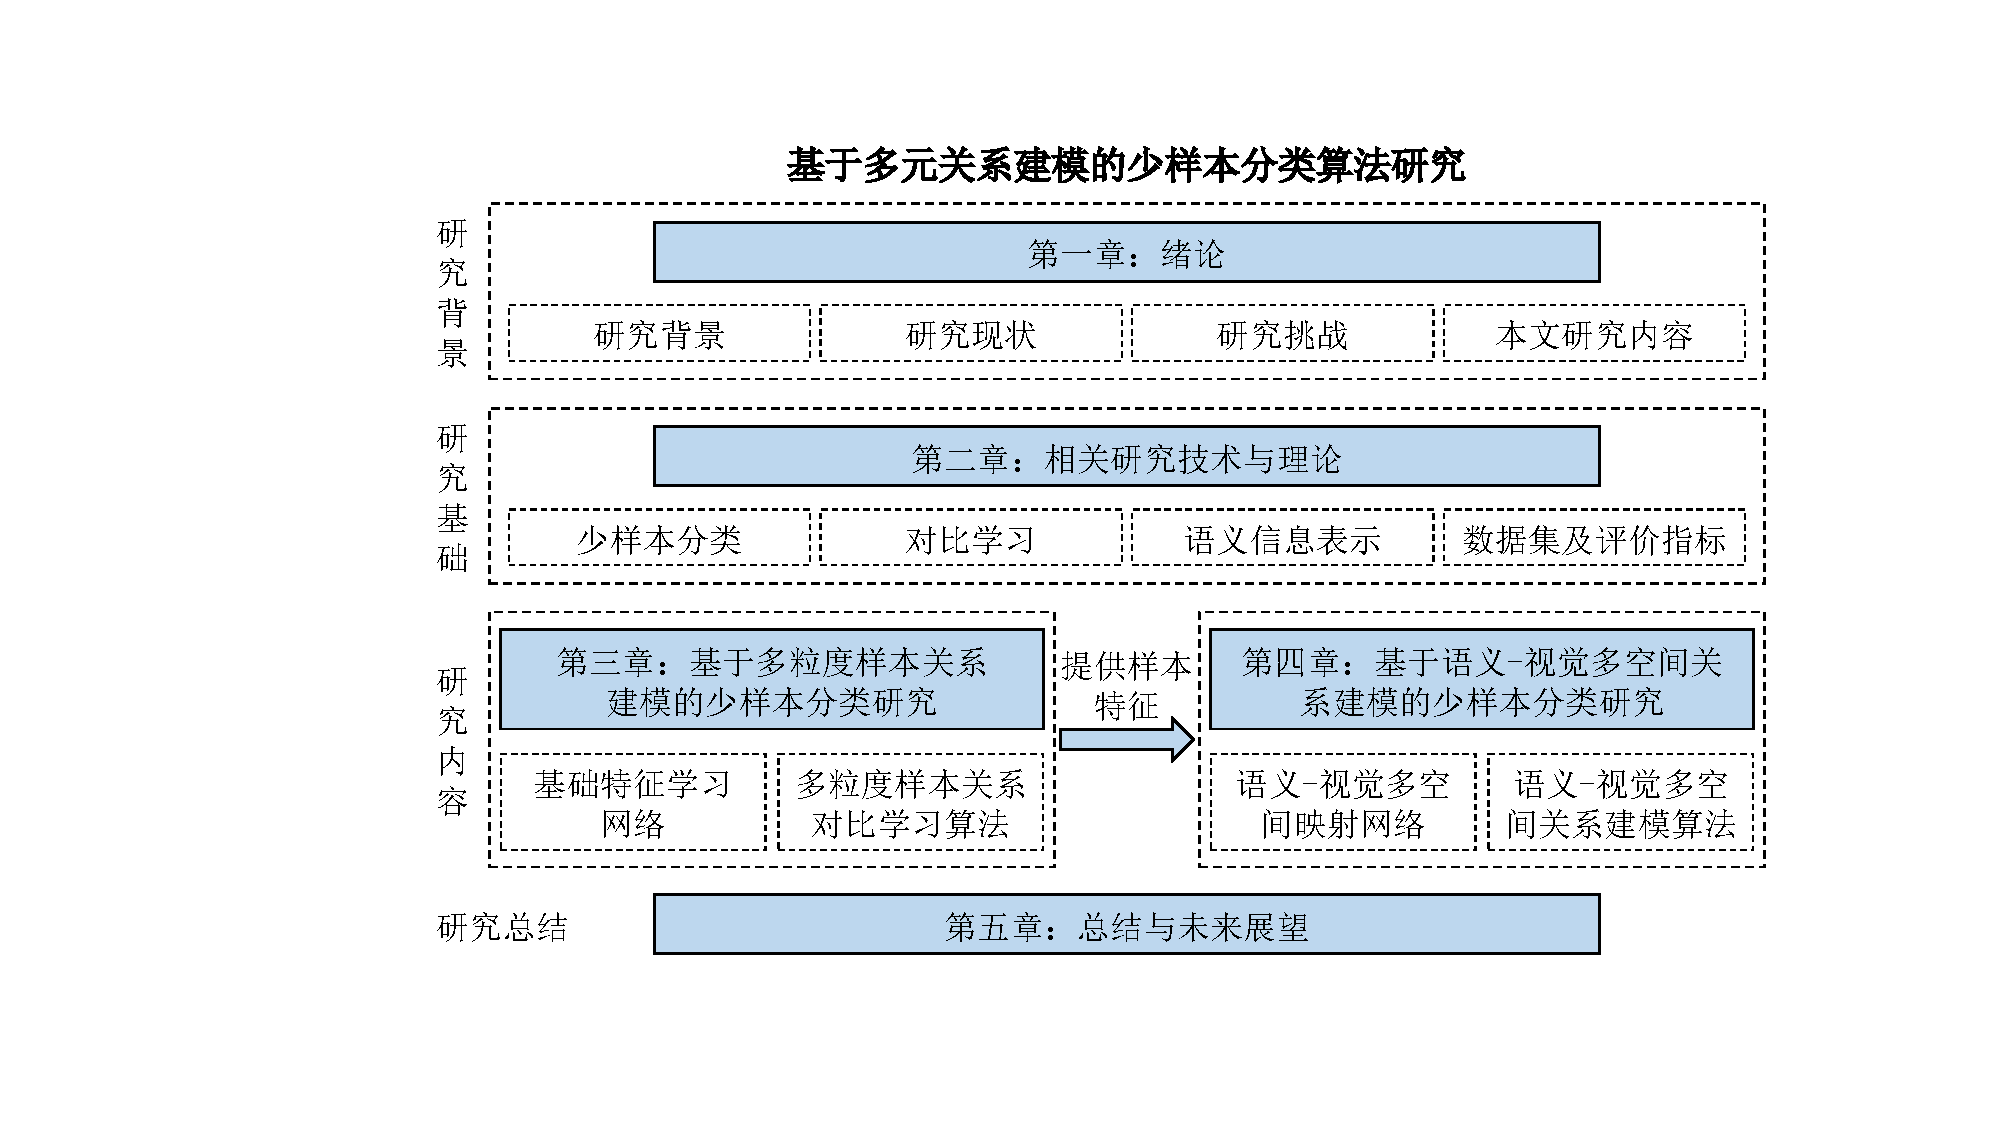
\includegraphics[width=1.0\columnwidth]{figures/组织结构.pdf}
    \bicaption[本文组织结构图]{本文组织结构图。}[The organizational structure of the paper]{The organizational structure of the paper.}
    \label{figure1: 组织结构}
\end{figure}

\section[\hspace{-2pt}本文组织结构]{{\heiti\zihao{-3} \hspace{-8pt}本文的组织结构}}\label{section1: 本文组织结构}

本文的组织结构图如图\ref{figure1: 组织结构}所示,共分为5个章节,各章节的介绍如下:

第一章:绪论。介绍少样本分类的研究背景和意义,并分析总结少样本分类算法的国内外研究现状及存在的挑战。最后对本文的研究内容和组织结构进行概述。

第二章:相关研究技术与理论。首先对少样本分类进行了进一步详细介绍,然后介绍本文方法中所使用到的对比学习技术以及语义信息表示,最后对本文实验所使用到的数据集及评价指标进行介绍。

第三章:基于多粒度样本关系建模的少样本分类研究。首先对部分现有少样本特征学习算法的不足进行分析,提出了基于多粒度样本关系对比学习的少样本特征学习算法(MGSRCL),随后详细介绍了针对不同粒度样本关系的建模方法,最后通过在四个基准数据集的大量实验证明了MGSRCL模型的有效性。

第四章:基于语义-视觉多空间关系建模的少样本分类研究。首先对基于语义的少样本分类算法进行分析介绍,提出了基于语义-视觉多空间关系建模的少样本特征适配算法(SVMSMA),然后介绍了SVMSMA模型的模型框架以及提出的跨模态分类和跨模态特征对齐模块,最后对所提方法进行了实验分析。

第五章:总结与未来展望。总结并分析了本文提出的基于多元关系建模的少样本分类算法研究的成果及不足,并对未来的研究方向与内容进行了展望。

